%%%% Paramétrage du cours %%%%
\def\xxactivite{Cours}
\def\xxauteur{\textsl{Xavier Pessoles}}


\def\xxnumchapitre{Chapitre 2 \vspace{.2cm}}
\def\xxchapitre{\hspace{.12cm} Rapidité des systèmes}

\def\xxcompetences{%
\textsl{%
\textbf{Savoirs et compétences :}\\
%\begin{itemize}[label=\ding{112},font=\color{bleuxp}] 
%\item \textit{Mod3.C2 : } pôles dominants et réduction de l’ordre du modèle : principe, justification
%\item \textit{Res2.C4 : } stabilité des SLCI : définition entrée bornée -- sortie bornée (EB -- SB)	
%\item \textit{Res2.C5 : } stabilité des SLCI : équation caractéristique	
%\item \textit{Res2.C6 : } stabilité des SLCI : position des pôles dans le plan complexe
%\item \textit{Res2.C7 : } stabilité des SLCI : marges de stabilité (de gain et de phase)
%\end{itemize}
}}


\def\xxfigures{
%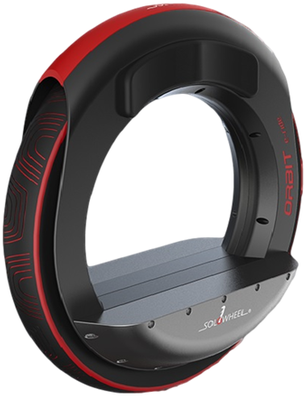
\includegraphics[width=3cm]{SoloWheel_Orbit}%
%\\
%\textit{SoloWheel Orbit.}
}%figues de la page de garde



\input{\repRel/Style/pagegarde_cours}

\setlength{\columnseprule}{.1pt}

\vspace{2cm}
\pagestyle{fancy}
%\thispagestyle{plain}


\section{Rappel : critère de rapidité dans le domaine temporel}

\subsection{Temps de réponse à 5\%}

\begin{methode}
\textbf{ -- Détermination du temps de réponse à $n\%$} (En pratique $n=5$).\\

\begin{enumerate}
\item Tracer sur le même graphe la consigne $e(t)$ et la réponse du système
$s(t)$.
\item Tracer la droite correspondant à la valeur asymptotique de $s(t)$.
\item Tracer la bande correspondant à une variation de $\pm n\%$ de la valeur
asymptotique.
\item Relever la dernière valeur à partir de laquelle $s(t)$ coupe la bande et
n'en sort plus.
\end{enumerate}
\end{methode}

\begin{center}
%\includestandalone{perf}
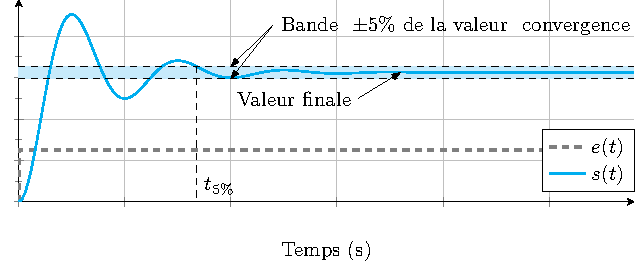
\includegraphics{perf}
\end{center}

\begin{resultat}
Plus le temps de réponse à 5\% d'un système est petit, plus le régime transitoire disparaît rapidement. 
\end{resultat}

\begin{exemple}
Donner le temps de réponse à 5\% de la réponse à un échelon donné dans la figure suivante. 


\begin{minipage}[c]{.5\linewidth}
\begin{center}
%\includestandalone{perf}
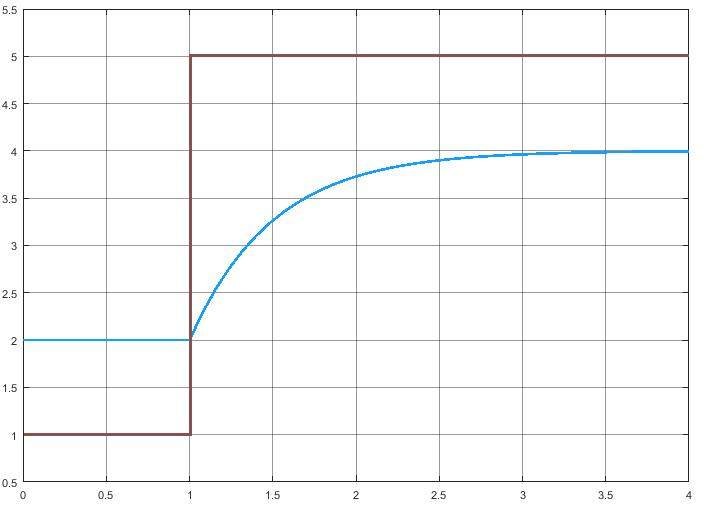
\includegraphics[width=8cm]{tr.jpg}
\end{center}
\end{minipage} \hfill
\begin{minipage}[c]{.4\linewidth}
Les pièges du temps de réponse à 5\% :
\begin{itemize}
\item le temps de réponse à 5\% se mesure à plus ou moins 5\% de la sortie (et pas de l'entrée). Ainsi, si le système est stable, le temps de réponse n'est \textbf{jamais l'infini};
\item si le signal ne part pas de 0 (en ordonnée), il faut réaliser la bande à $S_0+\Delta s \pm 0.05\Delta s$;
\item si le signal ne part pas de 0 (en abscisse), il faut tenir compte du décalage des temps.
\end{itemize}
\end{minipage} 
\end{exemple}

\subsection{Temps de montée}


\begin{minipage}[c]{.48\linewidth}
Pour caractériser la rapidité d'un système, on peut aussi utiliser le temps de montée. Il s'agit du temps nécessaire pour passer de 10\% à 90\% de la valeur finale. Ce temps de montée caractériser la << vivacité >> d'un système. 
\end{minipage} \hfill
\begin{minipage}[c]{.4\linewidth}
\begin{center}
%\includestandalone{perf}
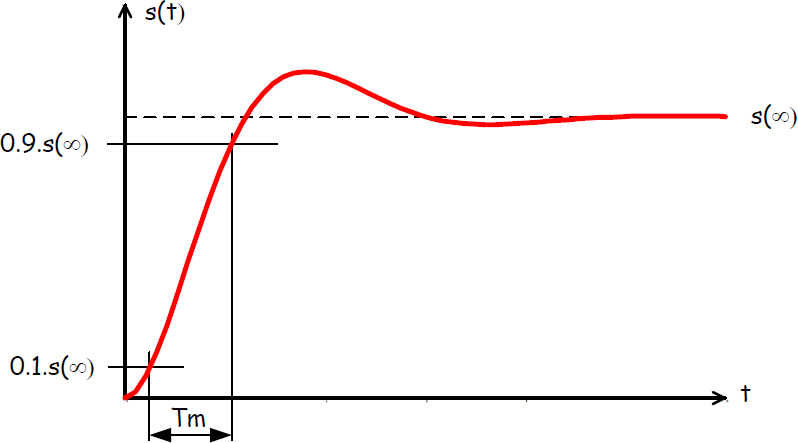
\includegraphics[width=\linewidth]{tm}
\end{center}
\end{minipage} 
\section{Rapidité des systèmes d'ordre 1 et d'ordre 2}
\subsection{Systèmes d'ordre 1}
Pour un système du premier ordre, le temps de réponse à 5\% est donné par $3\tau$.
\begin{resultat}
Pour un système du premier ordre, plus la constante de temps est petite, plus le système est rapide.
\end{resultat}

Soit un système du premier ordre bouclé avec un retour unitaire. L'expression de la FTBF est donnée par $\text{FTBF}(p)=\dfrac{K}{1+\tau p + K}$. La constante de temps est alors $\tau_{\text{BF}}=\dfrac{\tau}{1+K}$. 

\begin{resultat}
Pour un système du premier ordre bouclé (avec un retour unitaire), plus le gain statique est grand, plus le système est rapide. 
\end{resultat}

\subsection{Systèmes d'ordre 2}

\noindent\begin{minipage}[c]{.5\linewidth}
\begin{resultat}
Pour un système du second, à $\xi$ constant, plus la pulsation propre est grande, plus le système est rapide. 
\end{resultat} 



Soit un système du deuxième ordre bouclé avec un retour unitaire. En déterminant les caractéristiques de la FTBF, on obtient $K_{\text{BF}}=\dfrac{K}{1+K}$, $\omega_{\text{BF}}=\omega_0\sqrt{1+K}$, $\xi_{\text{BF}}=\dfrac{\xi}{1+K}$.


\begin{resultat}
\begin{itemize}
\item L'augmentation du gain de FTBO augmente la pulsation de la FTBF. 
\item L'augmentation du gain de FTBO diminue le coefficient d'amortissement. Suivant la valeur de $\xi{\text{BF}}$ le système peut devenir plus ou moins rapide.  
\end{itemize}
\end{resultat}

\end{minipage}\hfill
\begin{minipage}[c]{.47\linewidth}
\begin{center}
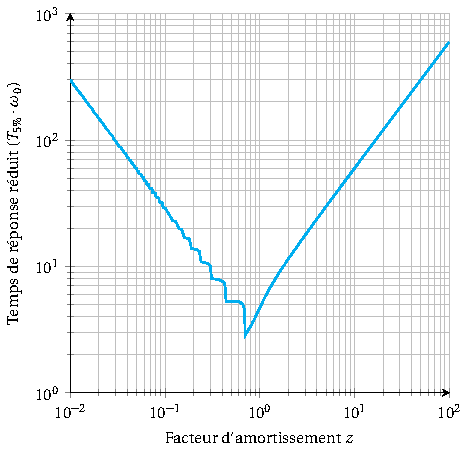
\includegraphics[width=\linewidth]{image7}
\end{center}
\end{minipage}

\section{Résultats dans le diagramme de Bode}


\noindent\begin{minipage}[c]{.48\linewidth}
\begin{resultat}
Plus la bande passante d'un système est élevée, plus le système est rapide.
\end{resultat}

\begin{center}
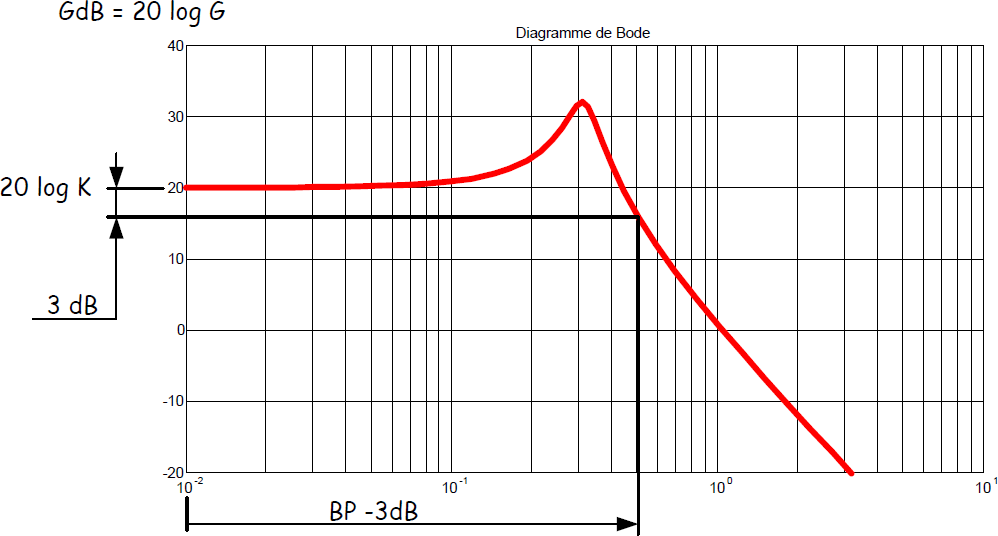
\includegraphics[height=4.5cm]{bandepassante}
\end{center}

\end{minipage} \hfill
\begin{minipage}[c]{.48\linewidth}
\begin{resultat}
Plus la pulsation de coupure à \SI{0}{dB} de la boucle ouverte est grande, plus le système asservi est rapide.
\end{resultat}


\begin{center}
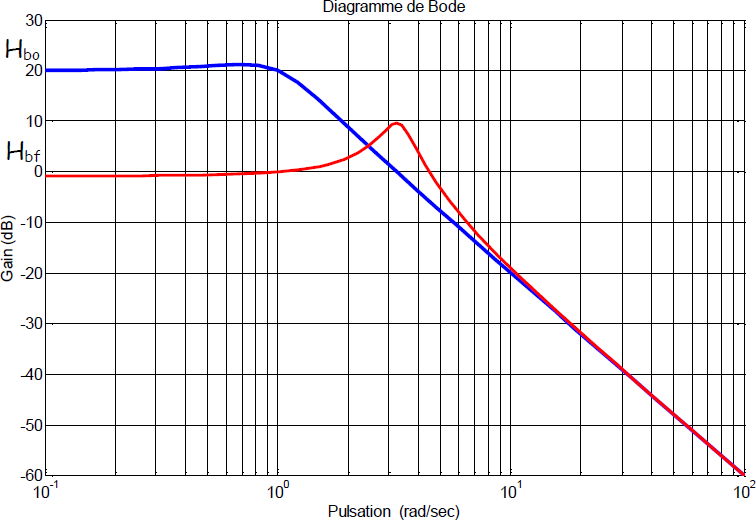
\includegraphics[height=4.5cm]{bobf}
\end{center}
\end{minipage}





\begin{thebibliography}{2}
   \bibitem[1]{ref1} Frédéric Mazet, {\it Cours d'automatique de deuxième année, Lycée Dumont Durville, Toulon.}
      \bibitem[2]{ref2} Florestan Mathurin, {\it Stabilité des SLCI, Lycée Bellevue, Toulouse, \url{http://florestan.mathurin.free.fr/}.}
\end{thebibliography}
